%\documentclass[10pt,a4paper]{article}
\documentclass[12pt,a4paper]{article}
\usepackage{graphicx,amsmath}
%\usepackage{subfigure}
\usepackage{float}
\usepackage[german]{babel}
\usepackage[utf8]{inputenc}
\setcounter{secnumdepth}{4}
\usepackage[top=2cm, bottom=2.5cm, left=3cm, right=3cm]{geometry}
\begin{document}


%\title{Bachelorarbeit}
%\author{Richard Kullmann}
%\date{02.06.2017}

\thispagestyle{empty}
%\setcounter{page}{2}
\newpage
\tableofcontents
\thispagestyle{empty}
\newpage
\pagenumbering{arabic}

\section{deterministisches Modell}
Durch die Wahl der Anfangsparameter im deterministischen Modell ohne bias-Strom kann beeinflusst werden, ob das System in den Gleichgewichtszustand oder auf den stabilen Grenzzyklus geht: 
\begin{figure}[H]
	\centering
	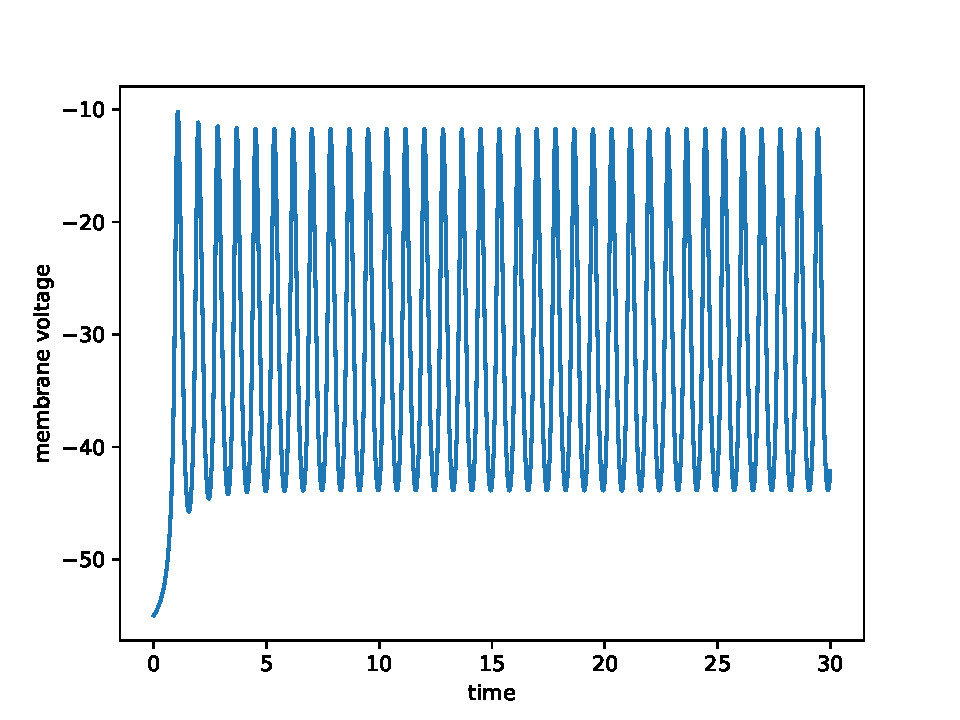
\includegraphics[scale=0.9]{inapi0d0.pdf} 
	\caption{Verhalten der Membranspannung mit burstenden Anfangsbedingungen}
	\label{burst}
\end{figure} 
\begin{figure}[H]
	\centering
	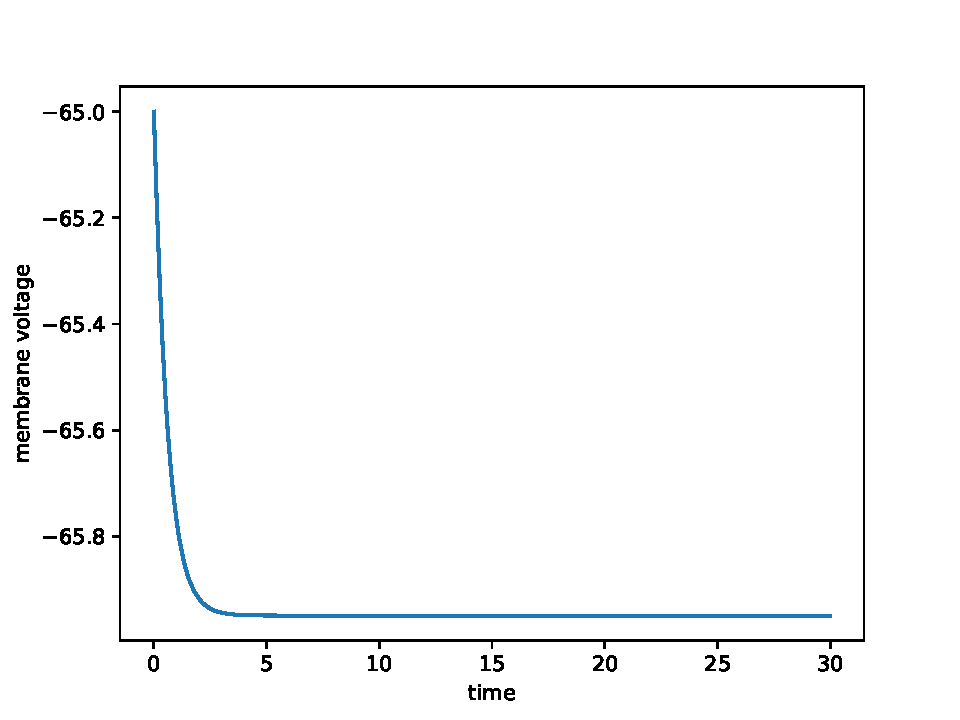
\includegraphics[scale=0.9]{inapnbi0d0.pdf} 
	\caption{Verhalten der Membranspannung mit nicht-burstenden Anfangsbedingungen}
	\label{noburst}
\end{figure}
Ob eine Kombination von Startparametern Bursten hervorruft, kann z.B. aus den Phasenporträts in master.pdf ermittelt werden.
\newpage
Die Evolution des Systems lässt sich auch gut am Phasendiagramm beobachten:
\begin{figure}[H]
	\centering
	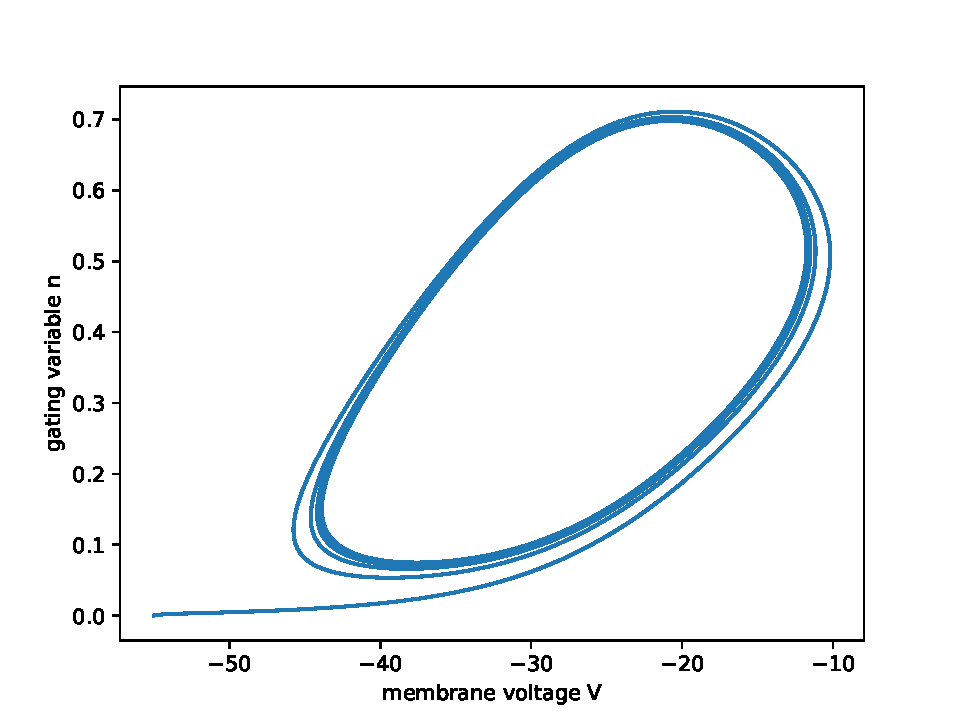
\includegraphics[scale=0.8]{inapi0d0p.pdf} 
	\caption{Beziehung zwischen Gatingvariable und Membranspannung bei burstenden Anfangsbedingungen}
	\label{burstp}
\end{figure} 
\begin{figure}[H]
	\centering
	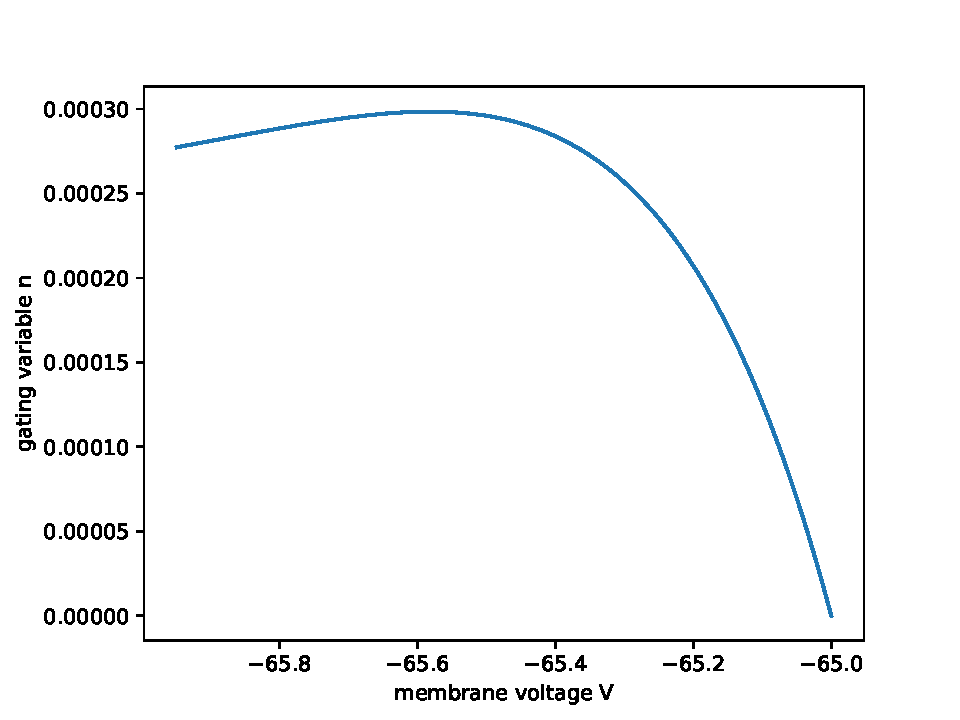
\includegraphics[scale=0.8]{inapnbi0d0p.pdf} 
	\caption{Beziehung zwischen Gatingvariable und Membranspannung bei nicht-burstenden Anfangsbedingungen}
	\label{noburstp}
\end{figure}
\section{Modell mit Rauschen}
Durch Einführung von Rauschen können Übergänge zwischen dem burstenden und dem Ruhezustand herbeigeführt werden. 
\begin{figure}[H]
	\centering
	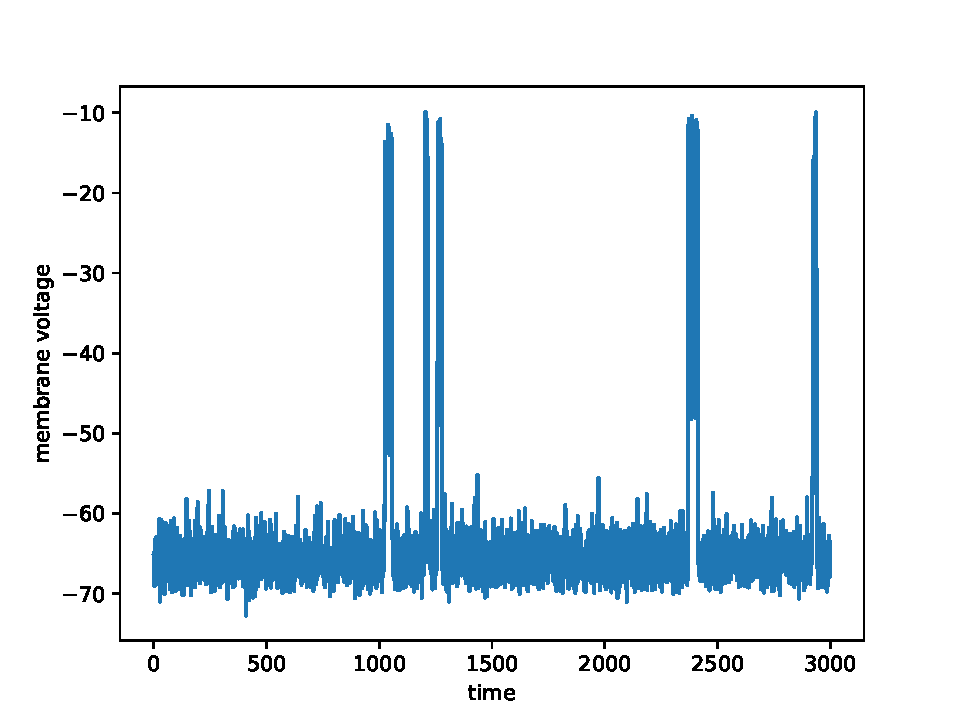
\includegraphics[scale=0.9]{inapni0d5.pdf} 
	\caption{Ohne Bias-Strom weist der Ruhezustand bei rauschinduzierten Übergängen längere Verweilzeiten auf}
	\label{i0d5}
\end{figure}
\begin{figure}[H]
	\centering
	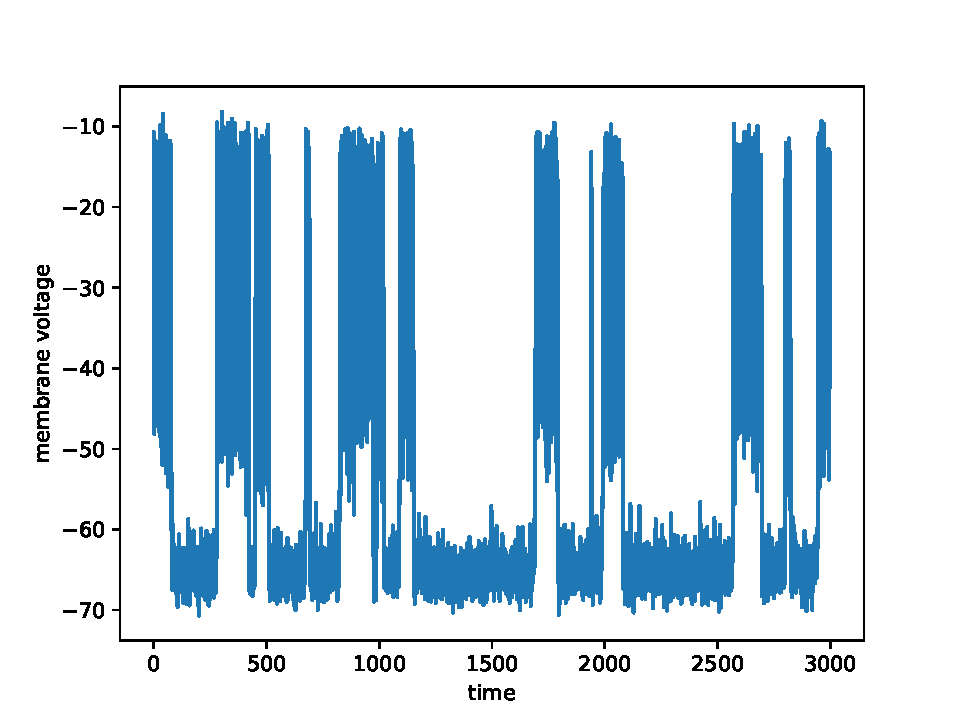
\includegraphics[scale=0.9]{inapi1d5.pdf} 
	\caption{Bei I=1 beobachtet weisen beide Zustände etwa gleiche Verweilzeiten auf}
	\label{i1d5}
\end{figure}
\begin{figure}[H]
	\centering
	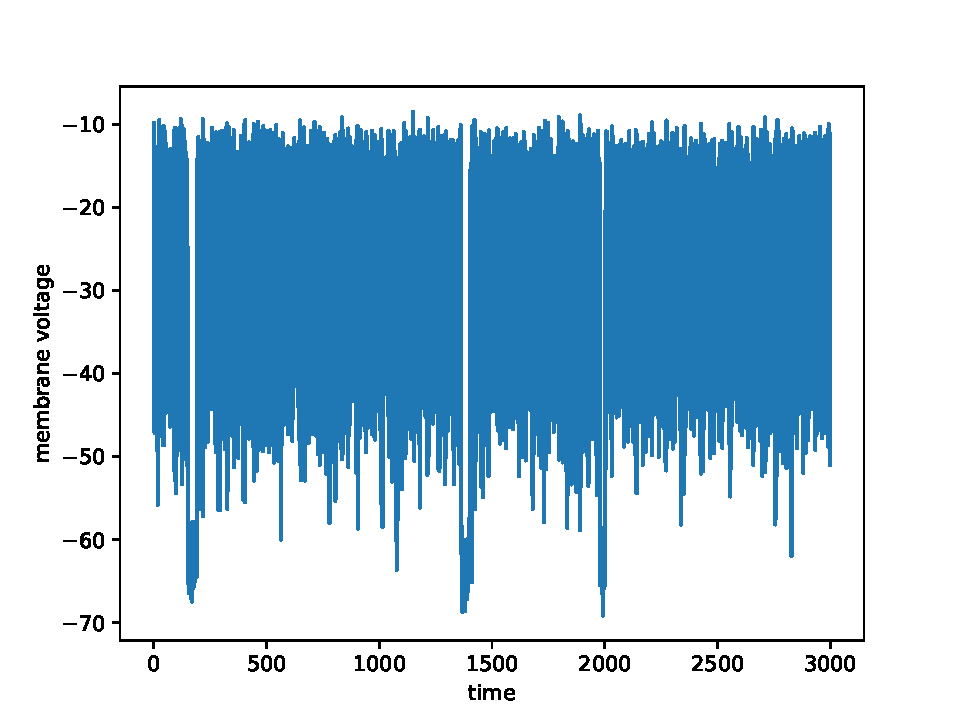
\includegraphics[scale=0.9]{inapi3d5.pdf} 
	\caption{Bei I=3 ist nahezu nur noch Bursten zu sehen}
	\label{i3d5}
\end{figure}
\end{document}